%//==============================--@--==============================//%

Os semicondutores são materiais que possuem propriedades elétricas intermediárias entre os isolantes e os condutores, e dispõem de uma propriedade única: a sua condutividade eléctrica aumenta com a temperatura, ao contrário dos metais, cuja condutividade diminui com a temperatura. 

O silício (Si) e o germânio (Ge) são dois exemplos bem conhecidos de semicondutores (ambos do grupo 14 da tabela periódica).

%//==============================--@--==============================//%
\subsection[1.1 Semicondutores intrínsecos e dopados]{\hspace*{0.075 em}\raisebox{0.2 em}{$\pmb{\drsh}$} Semicondutores intrínsecos e dopados}
\label{subsec:semiconductors-intrinsic-and-doped}

\begin{itemize}
    \item \textbf{Semicondutores intrínsecos:} Semicondutores puros, como o silício cristalino, que não possuem impurezas. A condutividade elétrica é determinada apenas pela concentração de portadores de carga intrínsecos, ou seja, eletrões e lacunas geradas pela quebra de ligações covalentes.
    
    \item \textbf{Semicondutores dopados:} Semicondutores obtidos a partir da adição intencional de impurezas (dopantes) ao material semicondutor. O processo de dopagem permite controlar as propriedades elétricas do material e aumentar a sua condutividade. Existem dois tipos principais de dopagem de semicondutores:
    \begin{itemize}[label=$\blacktriangle$]
        \item \textbf{Dopagem de tipo n:} Dopagem com impurezas que possuem mais eletrões de valência do que o material semicondutor (normalmente com elementos pentavalentes, como o fósforo no silício). Estes materiais apresentam uma maior concentração de eletrões, que são portadores de carga negativa.
        
        \item \textbf{Dopagem de tipo p:} Dopagem com impurezas que possuem menos eletrões de valência do que o material semicondutor (comummente elementos trivalentes, como o boro no silício). Estes materiais apresentam uma maior concentração de lacunas, que são portadoras de carga positiva.
    \end{itemize}
\end{itemize}

%//==============================--@--==============================//%
\subsubsection[1.1.1 Principio de funcionamento dos semicondutores]{$\pmb{\rightarrow}$ Principio de funcionamento dos semicondutores}

\begin{itemize}
	\item A temperaturas extremamente baixas (próximas de 0 K), tendem para um comportamento próximo ao dos isoladores dado que todas as ligações covalentes estão intactas (não há geração de eletrões livres e lacunas para conduzir corrente).
 
	\item À temperatura ambiente, a energia térmica provoca a quebra de algumas ligações covalentes, um processo conhecido como \underline{geração térmica}. Isto resulta em eletrões livres que podem conduzir corrente elétrica quando é aplicado um campo elétrico.
 
    \item Quando um eletrão deixa o seu átomo de origem, cria uma carga positiva (uma lacuna) de igual magnitude. Outros eletrões podem ser atraídos para esta lacuna e mover-se para a preencher, fazendo com que a lacuna se mova efetivamente através da estrutura cristalina. As lacunas também podem conduzir corrente elétrica.
 \end{itemize}

\vspace{-1.0em}
\begin{figure}[H]
    \centering
    \begin{minipage}{0.35\textwidth}
        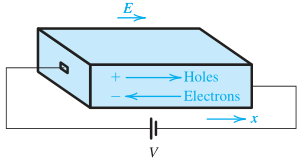
\includegraphics[width=1\textwidth]{img/1/bar-of-silicon.png}
    \end{minipage}
    \hfill
    \begin{minipage}{0.60\textwidth}
        \caption{``An electric field E established in a bar of silicon causes the holes to drift in the direction of E and the free electrons to drift in the opposite direction. Both the hole and electron drift currents are in the direction of E.''\cite{sedra-smith:microelectronic-circuits}}
    \end{minipage}
    \label{fig:bar-of-silicon}
\end{figure}

\renewcommand*{\thefootnote}{\fnsymbol{footnote}}
\footnotetext[4]{%
    À medida que a temperatura aumenta, mais ligações covalentes se rompem, o que resulta em mais pares eletrão-lacuna, aumentando a condutividade do silício.
}
\renewcommand*{\thefootnote}{\arabic{footnote}}

%//==============================--@--==============================//%
\subsection[1.2 Fluxo de corrente nos semicondutores]{\hspace*{0.075 em}\raisebox{0.2 em}{$\pmb{\drsh}$} Fluxo de corrente nos semicondutores}
\label{subsec:current-flow-semiconductors}

O fluxo de corrente nos semicondutores pode ser dividido em dois componentes principais: corrente de deriva e corrente de difusão.

\begin{itemize}[leftmargin=*]
    \item \textbf{Corrente de deriva}:
    \begin{itemize}
        \item[$($\textbf{?}$)$] Causada pelo movimento de portadores de carga (eletrões e lacunas) sob a influência de um campo elétrico externo.
        \item[$\blacktriangle$] A densidade de corrente de deriva, $J_{\textit{drift}}$, pode ser descrita pela fórmula:
        \begin{equation*}
            J_{\textit{drift}} = q(n \mu_n + p \mu_p)E
        \end{equation*}
        onde $q$ é a carga elementar, $n$ e $p$ são as concentrações de eletrões e lacunas (respetivamente), $\mu_n$ e $\mu_p$ são as mobilidades dos eletrões e lacunas, e $E$ é a intensidade do campo elétrico aplicado.
    \end{itemize}

    \item \textbf{Corrente de difusão}:
    \begin{itemize}
        \item[$($\textbf{?}$)$] Causada pelo movimento de portadores de carga devido a gradientes de concentração, ou seja, os portadores de carga movem-se de regiões de maior concentração para regiões de menor concentração.
        \item[$\blacktriangle$] A densidade de corrente de difusão para eletrões, $J_{n, \textit{diff}}$, e lacunas, $J_{p, \textit{diff}}$, pode ser descrita pelas fórmulas:
            \begin{align*}
                J_{n, \textit{diff}} &= -qD_n\frac{dn}{dx} \\
                J_{p, \textit{diff}} &= qD_p\frac{dp}{dx}
            \end{align*}
        onde $D_n$ e $D_p$ são os coeficientes de difusão para eletrões e lacunas, e $dn/dx$ e $dp/dx$ são os gradientes de concentração para eletrões e lacunas, respetivamente.
    \end{itemize}

    \item \textbf{Relação de Einstein}:
    \begin{itemize}
        \item[$($\textbf{?}$)$] Estabelece uma ligação entre o coeficiente de difusão e a mobilidade dos portadores de carga num semicondutor.
        \item[$\blacktriangle$] A relação para eletrões ($D_n$) e lacunas ($D_p$) é dada pelas fórmulas:
            \begin{align*}
                D_n &= \mu_n \frac{k T}{q} \\
                D_p &= \mu_p \frac{k T}{q}
            \end{align*}
        onde $k$ é a constante de Boltzmann, $T$ a temperatura absoluta em Kelvin e $q$ o valor da carga elementar.
        \item[$\blacktriangle$] Esta relação liga os processos de deriva e difusão dos semicondutores, uma vez que implica que o coeficiente de difusão é diretamente proporcional à mobilidade dos portadores de carga. É possível representar a relação sucintamente:
            $$
                \boxed{ \frac{D_n}{\mu_n} = \frac{D_p}{\mu_p} = V_T }
            $$
        onde $V_T \delequal kT/q$. O parâmetro $V_T$ é conhecido como a \textbf{tensão térmica}. 
        
        \textbf{Nota:} À temperatura ambiente, $T \simeq 300$K e $V_T \simeq 25$ mV.    
    \end{itemize}
\end{itemize}
    
%//==============================--@--==============================//%
\clearpage
\subsection[1.3 Junção pn]{\hspace*{0.075 em}\raisebox{0.2 em}{$\pmb{\drsh}$} Junção pn}
\label{subsec:pn-junction}

Uma junção pn é formada quando um semicondutor tipo p (com um excesso de lacunas) é colocado em contacto com um semicondutor tipo n (com um excesso de elétrões).

\begin{figure}[H]
    \centering
    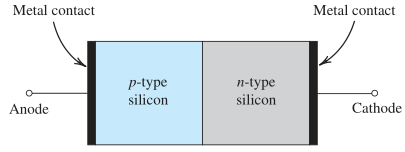
\includegraphics{img/1/simplified-pn-junction.png}
    \caption{``Simplified physical structure of the pn junction. (...)''\cite{sedra-smith:microelectronic-circuits}}
    \label{fig:simplified-pn-junction}
\end{figure}

\begin{figure}[ht] 
    \begin{subfigure}[b]{0.5\linewidth}
        \centering
        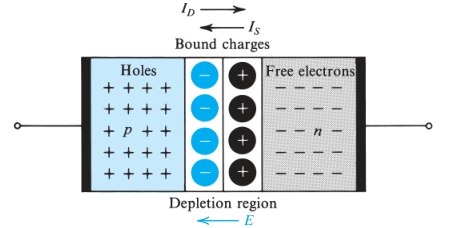
\includegraphics[width=1\linewidth]{img/1/pn-junction-OC.png}
        \caption{} 
        \label{fig:pn-junction-OC} 
    \end{subfigure}%% 
    \begin{subfigure}[b]{0.5\linewidth}
        \centering
        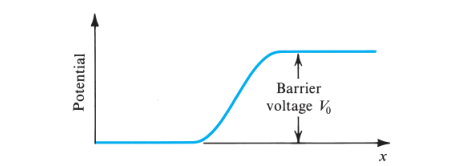
\includegraphics[width=1\linewidth]{img/1/pn-junction-potential-distrib.png} 
        \caption{} 
        \label{fig:pn-junction-potential-distrib} 
    \end{subfigure}  
    \caption{``(a) The pn junction with no applied voltage (open-circuited terminals). (b) The potential distribution along an axis perpendicular to the junction.''\cite{sedra-smith:microelectronic-circuits}}
    \label{fig:pn-junction}
\end{figure}

\vspace{-1em}
\begin{itemize}[leftmargin=*, noitemsep]
    \item \textbf{Corrente de Difusão ($I_D$):}
    \begin{itemize}[leftmargin=*, label=$\pmb{-}$]
        \item Devido à alta concentração de lacunas na região p e baixa concentração na região n, as lacunas difundem-se através da junção do lado p para o lado n.
        \item De maneira semelhante, os eletrões difundem-se através da junção do lado n para o lado p devido à sua alta concentração na região n e baixa concentração na região p.
        \item Estes dois componentes da corrente juntam-se para formar a corrente de difusão $I_D$, que flui do lado p para o lado n.
    \end{itemize}
    
    \item \textbf{Corrente de Deriva/Corrente de Saturação Inversa ($I_S$):}
    \begin{itemize}[leftmargin=*, label=$\pmb{-}$]
        \item Além de $I_D$, existe uma componente da corrente proveniente da deriva de portadores minoritários (\textit{minor carriers}) através da junção.
        \item As lacunas geradas termicamente na região n movem-se em direção à junção, e à beira da região de depleção, são influenciadas pelo campo elétrico, que as arrasta para o lado p.
        \item De maneira semelhante, os eletrões gerados termicamente na região p movem-se para a beira da região de depleção e são arrastados pelo campo elétrico para o lado n.
        \item Estes dois componentes da corrente---eletrões movidos por deriva de p para n e lacunas movidas por deriva de n para p---somam-se para formar a corrente de deriva $I_S$, que flui do lado n para o lado p da junção.
        \item A corrente de deriva $I_S$ é fortemente dependente da temperatura mas independente da tensão da região de depleção $V_0$ $[$que veremos em seguida$]$.
    \end{itemize}
\end{itemize}

\newpage
\begin{itemize}[leftmargin=*, nolistsep]
    \item \textbf{Depletion region:}
    \begin{itemize}[label=$\blacktriangle$, leftmargin=*]
        \item Quando uma junção pn é formada, eletrões da região do tipo n (com excesso de eletrões) difundem-se na região do tipo p (com excesso de lacunas) devido ao gradiente de concentração (\hyperref[subsec:current-flow-semiconductors]{rever fluxo de corrente nos semicondutores}).
        \item Estes eletrões recombinam-se com as lacunas disponíveis na região do tipo p, criando uma região em torno da junção onde os portadores de carga móveis estão reduzidos. Essa região é chamada de \underline{região de depleção} ou \underline{camada de depleção}.
        \item A região de depleção tem uma largura que depende da concentração de dopagem de ambos os materiais do tipo p e do tipo n e da tensão aplicada através da junção. Atua como uma barreira ao fluxo de portadores de carga através da junção sob polarização inversa (\textit{reverse bias}).
    \end{itemize}

    \item \textbf{Built-in potential:}
    \begin{itemize}[label=$\blacktriangle$, leftmargin=*]
    \item À medida que os eletrões se difundem através da junção e se recombinam com as lacunas, deixam para trás iões doadores positivamente carregados na região do tipo n e iões aceitadores negativamente carregados na região do tipo p.
    \item Estes átomos doadores e aceitadores, ionizados e imóveis, criam um campo elétrico que se opõe à difusão adicional dos portadores de carga, impedindo a neutralização completa das impurezas de dopagem.
    \item A diferença de potencial gerada por este campo elétrico é chamada de \textit{built-in potential}. Esta tensão atua como uma barreira que deve ser superada por uma tensão externa para que os portadores de carga atravessem a junção em polarização direta (\textit{forward bias}). 
    
    A \textbf{barrier voltage} pode ser dada por (``$[$with$]$ no external voltage applied $[$...$]$''\cite{sedra-smith:microelectronic-circuits}):
    $$
        V_0 = V_T\, \ln\left(\frac{N_A N_D}{n^{2}_{i}}\right)
    $$
    onde $N_A$ e $N_D$ são as concentrações de dopagem do lado p e do lado n da junção (respetivamente); e $n^{2}_{i} \delequal$ produto da concentração de lacunas e de eletrões livres.
    \end{itemize}

    \item \textbf{Forward bias and reverse bias:}
    \begin{itemize}[label=$\blacktriangle$, leftmargin=*]
        \item O comportamento de uma junção pn depende da polaridade da tensão externa aplicada. Há duas condições: polarização direta e polarização reversa.
        \begin{itemize}[label=\rule{1ex}{1ex}, leftmargin=*]
            \item \textbf{Forward bias (polarização direta):}
            \begin{itemize}[label=$\pmb{-}$]
                \item Na polarização direta, a região do tipo p é conectada ao terminal positivo, e a região do tipo n é conectada ao terminal negativo da fonte de tensão.
                \item Esta tensão externa reduz a barreira de potencial criada pelo \textit{built-in potential}, permitindo que os portadores de carga (lacunas da região do tipo p e eletrões da região do tipo n) atravessem a junção.
                \item A corrente aumenta rapidamente com a tensão aplicada, resultando num fluxo de corrente unidirecional.
            \end{itemize}
        \end{itemize}
        
        \begin{itemize}[label=\rule{1ex}{1ex}, leftmargin=*]
            \item \textbf{Reverse bias (polarização inversa):}
            \begin{itemize}[label=$\pmb{-}$]
                \item Na polarização inversa, a região do tipo p é conectada ao terminal negativo, e a região do tipo n é conectada ao terminal positivo da fonte de tensão.
                \item Esta tensão externa aumenta a barreira de potencial, impedindo o fluxo de portadores de carga através da junção.
                \item A corrente é insignificante, tipicamente limitada a uma pequena corrente de saturação inversa devido à presença de portadores minoritários e portadores gerados termicamente.
            \end{itemize}
        \end{itemize}
    \end{itemize}
\end{itemize}

%//==============================--@--==============================//%